\begin{landscape}
\begingroup
\fontsize{10}{13}\selectfont
\fancyhead[L]{\small POSTHUMOUS PAPERS AND CORRESPONDENCE}
\renewcommand{\headrulewidth}{0pt}
\par\medskip
\pdfbookmark[2]{Posthumous Papers VII [3]}{pallas-VII-letters3}
\begin{center}[3.]\par\medskip
\textsc{Gauss} to \textsc{Encke}, Göttingen, 7 November 1816.
\end{center}
\par\noindent\hspace*{\parindent}Taking up your kind offer .\ .\ .\ .\ .\ I am sending you
today some calculations for the perturbations of Pallas. By way of explanation
I will first indicate what remains to be done. There are three kinds of operation:
\par\noindent\hspace*{\parindent}The \textls[100]{first operation} is already quite complete, so there is no need
to describe it here in greater detail.
\par\noindent\hspace*{\parindent}By the \textls[100]{second operation} I mean the calculation of 24 values of a
function of the form
\[
\odot)\qquad
\begin{aligned}
&a+a'\cos x+a''\cos2x+a'''\cos3x+\text{etc.}+a^{\mathrm{XII}}\cos12x\\
&\quad+b'\sin x+b''\sin2x+b'''\sin3x+\text{etc.}+b^{\mathrm{XII}}\sin12x
\end{aligned}
\]
\noindent for \(x=0^0\), \(x=15^0\), \(x=30^0\) etc. up to \(x=345^0\). This operation would have
to be carried out 126 times in all, of which 62 are still outstanding.
\par\noindent\hspace*{\parindent}By the \textls[100]{third operation} I mean determining \(\log r\) and \(\varphi\) 24 times from
\[
\begin{aligned}
r\cos\varphi&=P\\
r\sin\varphi&=Q
\end{aligned}
\]
\SourceLeaf{575}
\noindent where \(P\) and \(Q\) are given quantities (each calculated from the form \(\odot\)).
This operation had to be carried out 60 times in all. 48 are still outstanding.
\par\noindent\hspace*{\parindent}Today I am sending you the data on 8 small sheets for carrying out the third
operation 8 times. Each \(P\) is obtained from the numbers at the bottom of
the side headed \(\sin A\) and each \(Q\) from the numbers on the other side,
headed \(\cos A\), in the following way. Each \(P\) consists of two parts
(which come from the cosine and sine terms, respectively). These
two parts are given directly for 13 values in
this order
\providecommand{\VIIthreeStars}[1]{\begin{array}{@{}c@{}}\ast\\\ast\end{array}\;#1}
\begingroup\small
\[
\begin{aligned}
&\begin{array}{c|c|c|c|c|c|c}
\VIIthreeStars{0^0}&\VIIthreeStars{30^0}&\VIIthreeStars{60^0}&\VIIthreeStars{90^0}&\VIIthreeStars{120^0}&\VIIthreeStars{150^0}&\VIIthreeStars{180^0}
\end{array}\\[1ex]
&\begin{array}{c|c|c|c|c|c|}
\VIIthreeStars{15^0}&\VIIthreeStars{45^0}&\VIIthreeStars{75^0}&\VIIthreeStars{105^0}&\VIIthreeStars{135^0}&\VIIthreeStars{165^0}
\end{array}
\end{aligned}
\]
\endgroup
\par\noindent\hspace*{\parindent}After that the same order is followed in reverse, always taking the second
(sine) part with the opposite sign. For example, on the first sheet we
have
\[
\begin{array}{r|r|r}
x&P&Q\\
0^0&+39{,}5723&-24{,}3180\\
15^0&+18{,}4497&-17{,}9717\\
30^0&-1{,}5499&-18{,}3889\\
\vdots&\vdots&\vdots\\
180^0&-6{,}8889&-39{,}1004\\
195^0&-5{,}3849&-40{,}6708\\
210^0&-2{,}6665&-42{,}6184\\
\vdots&\vdots&\vdots
\end{array}
\]
\par\noindent I carry out a complete calculation of the second operation on a single octavo page
in this format for the following values
\begingroup\renewcommand{\arraystretch}{1.8}\setlength{\tabcolsep}{13pt}
\begin{center}
\begin{tabular}{|c|c|c|c|c|c|}
\hline
\(0^0\)&\(15^0\)&\(30^0\)&\(45^0\)&\(60^0\)&\(75^0\)\\\hline
\(90^0\)&\(105^0\)&etc.&&&\\\hline
\rule{0pt}{1.8em}&&&&&\\\hline
\rule{0pt}{1.8em}&&&&&\\\hline
\end{tabular}
\end{center}\endgroup
\SourceLeaf{576}
\par\noindent In my way of doing the calculation, the first square would look like this:
\begin{center}
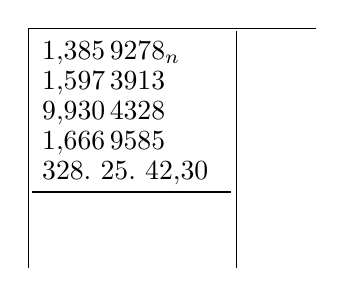
\begin{tikzpicture}[x=1cm,y=1cm]
\draw (0,-.75)--(0,2.30)--(3.65,2.30);
\draw (2.65,-.75)--(2.65,2.27);
\draw (.05,.22)--(2.58,.22);
\node[anchor=west,inner sep=0pt] at (.17,1.98) {\(1{,}385\,9278_n\)};
\node[anchor=west,inner sep=0pt] at (.17,1.60) {\(1{,}597\,3913\)};
\node[anchor=west,inner sep=0pt] at (.17,1.22) {\(9{,}930\,4328\)};
\node[anchor=west,inner sep=0pt] at (.17,.84) {\(1{,}666\,9585\)};
\node[anchor=west,inner sep=0pt] at (.17,.46) {\(328.\ 25.\ 42{,}30\)};
\end{tikzpicture}
\end{center}
\par\noindent I omit \(\log\operatorname{tang}\varphi\) here. If this is inconvenient for you,
please include it.
Then please send me all these details so that
I can compare the calculations more easily if
differences show up anywhere. There is no need,
however, to be excessively scrupulous in calculating. The calculations I have now assigned you will therefore fill 4 octavo leaves. I would like you to use both sides of the paper so that I do not have too many
papers to keep track of. — Incidentally, I carried out all the calculations to 7 decimal places.
\par\noindent\hspace*{\parindent}The 8 sheets I am sending you also contain 16 complete instances of the second operation in the form I use. To find your
way around them, a careful analysis of a form of this kind will serve you
better than lengthy instructions. I will only note that the
upper half of each sheet always contains the calculations for the cosine parts and
the lower half those for the sine parts. To help you decipher them,
the page .\ .\ .\ .\ .\ may serve as an example. The formula \(\odot\) was
\[
\begin{array}{r@{\;}l@{\qquad}r@{\;}l}
+82{,}2072&&&\\
-4{,}7425&\cos x&-13{,}7875&\sin x\\
-2{,}6435&\cos2x&-7{,}5676&\sin2x\\
-0{,}6305&\cos3x&-3{,}8103&\sin3x\\
+0{,}9201&\cos4x&-1{,}9322&\sin4x\\
+1{,}5425&\cos5x&-0{,}5853&\sin5x\\
+0{,}8559&\cos6x&-0{,}2174&\sin6x\\
+0{,}4068&\cos7x&-0{,}0161&\sin7x\\
+0{,}1649&\cos8x&+0{,}0436&\sin8x\\
\multicolumn{2}{c}{0}&\multicolumn{2}{c}{0}\\
\multicolumn{2}{c}{0}&\multicolumn{2}{c}{0}\\
\multicolumn{2}{c}{0}&\multicolumn{2}{c}{0}\\
\multicolumn{2}{c}{0}&\multicolumn{2}{c}{0}
\end{array}
\]
\SourceLeaf{577}
\begin{center}\small
\begin{tabular}{c|c}
\shortstack{The frequently occurring numbers}&\shortstack{are constant logarithms of}\\[.6ex]
\(9{,}787\,0156\)&\(\BareRoot{\frac38}\)\\[.5ex]
\(9{,}849\,4850\)&\(\BareRoot{\frac12}\)\\[.5ex]
\(9{,}937\,5306\)&\(\BareRoot{\frac34}\)
\end{tabular}
\end{center}
\par\noindent For the two parts of the operation marked with
\tikz[baseline=-.1em,x=1em,y=1em]{\draw (0,0) rectangle (.72,.72);}
\tikz[baseline=-.1em,x=1em,y=1em]{\draw (0,0) rectangle (.72,.72);\draw (.07,.07) rectangle (.65,.65);}
I always keep
this form at hand:
\begin{center}
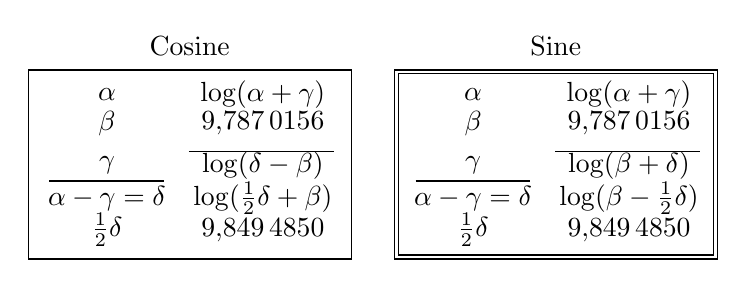
\begin{tikzpicture}[x=1cm,y=1cm]
\node at (2.05,2.55) {Cosine};
\node at (6.70,2.55) {Sine};
\draw (0,-.15) rectangle (4.10,2.25);
\draw (4.65,-.15) rectangle (8.75,2.25);
\draw (4.70,-.10) rectangle (8.70,2.20);
\draw (.27,.84)--(1.72,.84);
\draw (2.04,1.22)--(3.88,1.22);
\draw (4.92,.84)--(6.37,.84);
\draw (6.69,1.22)--(8.53,1.22);
\node at (1.00,1.94) {\(\alpha\)};
\node at (1.00,1.57) {\(\beta\)};
\node at (1.00,1.04) {\(\gamma\)};
\node at (1.00,.62) {\(\alpha-\gamma=\delta\)};
\node at (1.00,.22) {\(\frac12\delta\)};
\node at (2.98,1.94) {\(\log(\alpha+\gamma)\)};
\node at (2.98,1.57) {\(9{,}787\,0156\)};
\node at (2.98,1.04) {\(\log(\delta-\beta)\)};
\node at (2.98,.62) {\(\log(\frac12\delta+\beta)\)};
\node at (2.98,.22) {\(9{,}849\,4850\)};
\node at (5.65,1.94) {\(\alpha\)};
\node at (5.65,1.57) {\(\beta\)};
\node at (5.65,1.04) {\(\gamma\)};
\node at (5.65,.62) {\(\alpha-\gamma=\delta\)};
\node at (5.65,.22) {\(\frac12\delta\)};
\node at (7.63,1.94) {\(\log(\alpha+\gamma)\)};
\node at (7.63,1.57) {\(9{,}787\,0156\)};
\node at (7.63,1.04) {\(\log(\beta+\delta)\)};
\node at (7.63,.62) {\(\log(\beta-\frac12\delta)\)};
\node at (7.63,.22) {\(9{,}849\,4850\)};
\end{tikzpicture}
\end{center}
\par\noindent The rest is easy to learn by heart.
\par\noindent\hspace*{\parindent}Once you have worked everything out, please carry out the following
two applications for the time being: .\ .\ .\ .\ .
\par\medskip
\begin{center}\textsc{Gauss} to \textsc{Encke}, Göttingen, 3 March 1817.\end{center}
\par\noindent\hspace*{\parindent}.\ .\ .\ .\ .\ Four elements, the longitude of perihelion, the angle of eccentricity, the inclination
of the orbit, and the longitude of the node, are now fully settled and entered. What remains to be done on the 5th element, the epoch of longitude,
I have reserved for myself. For the 6th, however, the logarithm
of the semimajor axis, I take the liberty of asking for your help once again.
\par\noindent .\ .\ .\ .\ .
\clearpage
\endgroup
\end{landscape}
